\documentclass[border=10pt, varwidth=20cm]{standalone}
\usepackage[utf8]{inputenc}
\usepackage[T1]{fontenc}
\usepackage{tikz}
\usetikzlibrary{arrows.meta}

\begin{document}

    \centering

    % --- BLOCO 1: 4-ésimas raízes (Esquerda) ---
    \begin{minipage}{0.45\linewidth}
        \centering
        \begin{tikzpicture}[scale=1.8]
            \def\R{1}
            \draw[gray, thin, dashed] (0,0) circle (\R);
            \draw[->, >=stealth, gray!50] (-1.2,0) -- (1.2,0) node[right] {\tiny Re};
            \draw[->, >=stealth, gray!50] (0,-1.2) -- (0,1.2) node[above] {\tiny Im};
            
            \foreach \k in {0,1,2,3} {
                \coordinate (Q\k) at ({\k*360/4}:\R);
                \fill (Q\k) circle (1.5pt);
            }
            
            \node[above right] at (Q0) {\tiny $1$};
            \node[above right] at (Q1) {\tiny $\zeta = i$};
            \node[above left] at (Q2) {\tiny $\zeta^2 = -1$};
            \node[below left] at (Q3) {\tiny $\zeta^3 = -i$};
            
            \draw[blue!30, thin] (Q0) -- (Q2);
            \draw[blue!30, thin] (Q1) -- (Q3);
        \end{tikzpicture}
    \end{minipage}
    \hfill % Espaço entre as figuras
    % --- BLOCO 2: 8-ésimas raízes (Direita) ---
    \begin{minipage}{0.45\linewidth}
        \centering
        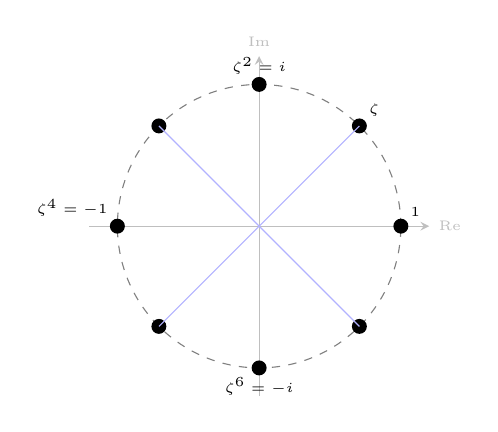
\begin{tikzpicture}[scale=1.8]
            \def\R{1}
            \draw[gray, thin, dashed] (0,0) circle (\R);
            \draw[->, >=stealth, gray!50] (-1.2,0) -- (1.2,0) node[right] {\tiny Re};
            \draw[->, >=stealth, gray!50] (0,-1.2) -- (0,1.2) node[above] {\tiny Im};
            
            \foreach \k in {0,...,7} {
                \coordinate (P\k) at ({\k*360/8}:\R);
                \fill (P\k) circle (1.5pt);
            }
            
            \node[above right] at (P0) {\tiny $1$};
            \node[above right] at (P1) {\tiny $\zeta$};
            \node[above] at (P2) {\tiny $\zeta^2 = i$};
            \node[above left] at (P4) {\tiny $\zeta^4 = -1$};
            \node[below] at (P6) {\tiny $\zeta^6 = -i$};
            
            \draw[blue!30, thin] (P1) -- (P5);
            \draw[blue!30, thin] (P3) -- (P7);
        \end{tikzpicture}
    \end{minipage}

\end{document}
    \begin{subfigure}[b]{0.48\textwidth}
        \centering
        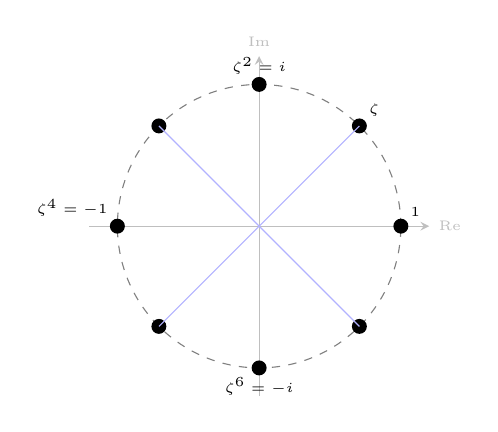
\begin{tikzpicture}[scale=1.8]
            \def\R{1}
            \draw[gray, thin, dashed] (0,0) circle (\R);
            \draw[->, >=stealth, gray!50] (-1.2,0) -- (1.2,0) node[right] {\tiny Re};
            \draw[->, >=stealth, gray!50] (0,-1.2) -- (0,1.2) node[above] {\tiny Im};
            
            \foreach \k in {0,...,7} {
                \coordinate (P\k) at ({\k*360/8}:\R);
                \fill (P\k) circle (1.5pt);
            }
            
            \node[above right] at (P0) {\tiny $1$};
            \node[above right] at (P1) {\tiny $\zeta$};
            \node[above] at (P2) {\tiny $\zeta^2 = i$};
            \node[above left] at (P4) {\tiny $\zeta^4 = -1$};
            \node[below] at (P6) {\tiny $\zeta^6 = -i$};
            
            \draw[blue!30, thin] (P1) -- (P5);
                \draw[blue!30, thin] (P3) -- (P7);
        \end{tikzpicture}
        \caption{8-ésimas raízes da unidade}
        \label{fig:raizes_8}
    \end{subfigure}
 